\chapter{Distorsione prospettica}
\label{sec:prospettiva}

\textbf{TODO: Continua}
Una camera acquisisce un'immagine catturando la luce proveniente dalla scena su di un sensore posto dietro un'apertura \textbf{NOME DI APERTURA}.
Per focalizzare i raggi di luce è utilizzata una lente.
Queste lenti introducono una distorsione radiale nell'immagine catturata, che dipende dalla curvatura della lente.
In alcuni casi tale distorsione è particolarmente intensa, ed è necessario correggerla prima di affrontare la distorsione prospettica, ma nella maggioranza dei casi questa non è notevole e può essere ignorata.

L'operazione di cattura dell'immagine può quindi essere modellata come proiezione dello spazio reale su un piano immagine, in cui i raggi di luce corrispondono alle linee di proiezione.
Per la correttezza del nostro modello è importante mantenere il rapporto tra lunghezza focale e la dimensione dei pixel, e la posizione dell'immagine rispetto all'asse della camera.
Non è quindi necessario che la distanza tra immagine e camera nel nostro modello corrisponda a quella tra il sensore e la lente nella realtà, ma può essere scelta in modo da ottenere misure più agevoli per i calcoli.
Comunemente si utilizza 1 unità come dimensione dei pixel dell'immagine, e la lunghezza focale si esprime in pixel.
Così facendo è possibile utilizzare qualsiasi unità di misura desiderata per la realtà senza dover modificare le coordinate dei punti dell'immagine.
Un'altra scelta comune per semplificare i calcoli è quella di porre l'origine degli assi delle coordinate al centro dell'immagine, orientare l'asse $x$ con le righe dell'immagine, l'asse $y$ con le colonne, e l'asse $z$ con l'asse ottico della camera, che è la linea che passa tra la camera e il centro dell'immagine.

Come espresso nella sezione \ref{sec:funzionalita-prospettiva} a noi interessa solamente ricorstruire ciò che accade sulla strada e ignoriamo il resto della scena.
Possiamo approssimare la strada con un piano, che chiamiamo piano stradale.
L'operazione che dobbiamo eseguire per correggere la distorsione prospettica si riduce così dalla proiezione da immagine a spazio reale tridimensionale a una proiezione da immagine a piano bidimensionale (fig \ref{fig:camera coords}).
Questa operazione non è lineare in coordinate cartesiane, ma diventa lineare se si utilizzano coordinate omogenee ed è quindi possibile definire una matrice di trasformazione.

\begin{figure}
    \caption{Modello con coordinate}
    \label{fig:camera coords}
    \centering
    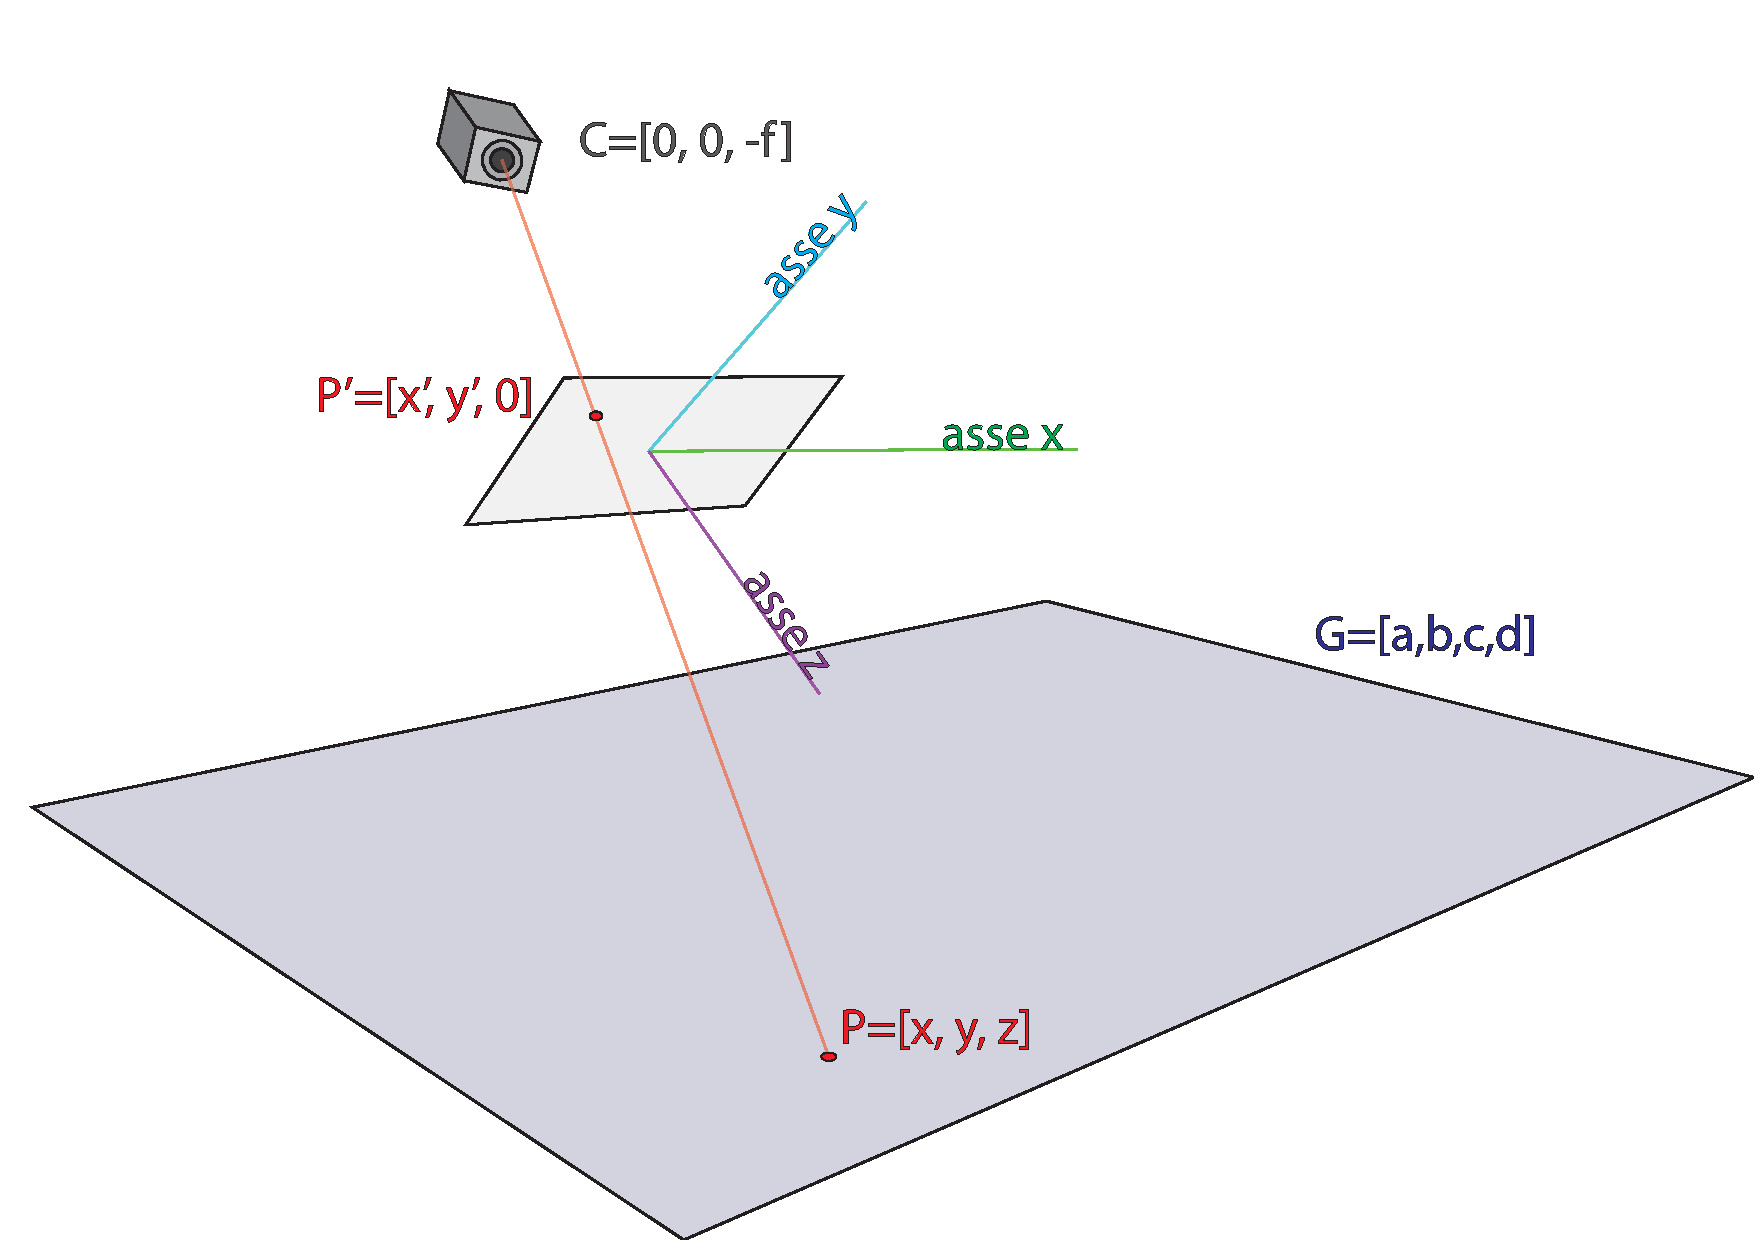
\includegraphics[width=\textwidth]{images/camera coords.pdf}
\end{figure}

È possibile definire tale matrice direttamente, ma è anche possibile definirla come combinazione di trasformazioni.
Tutte le trasformazioni affini sono componibili in coordinate omogenee, ed abbiamo quindi accesso a traslazione, rotazione e scalatura, a cui aggiungiamo la trasformazione di proiezione.
La trasformazione di proiezione prende le coordinate di un punto sull'immagine e dato un piano restituisce la posizione reale del punto immagine proiettato sul piano utilizzando la camera come proiettore.
Dato che le coordinate sono omogenee e non cartesiane il punto immagine è espresso con 3 coordinate e il punto reale trovato con 4 coordinate.
La trasformazione di proiezione è rappresentata con la matrice \ref{eq:projmat}:
\begin{equation}
    \label{eq:projmat}
    \begin{bmatrix}
        cf - d & 0      & 0   \\
        0      & cf - d & 0   \\
        -fa    & -fb    & -fd \\
        a      & b      & cf  \\
    \end{bmatrix}
\end{equation}
Dove:
\begin{itemize}
    \item il piano stradale è espresso come $ax + by + cz + d$, oppure $[a, b, c, d]^T$
    \item la lunghezza focale della camera è $f$
\end{itemize}

\textbf{TODO: bla bla spiega combinazione}
\begin{equation}
    \begin{aligned}
        O & = I^{-1} \cdot [0, 0, 0, 1]                       \\
        G & = T_{(O)}^{-1T} \cdot I_R^{-1} \cdot [0, 0, 1, 0] \\
        M & =
        \begin{bsmallmatrix}
            1 & 0 & 0 & 0 \\
            0 & 1 & 0 & 0 \\
            0 & 0 & 0 & 1 \\
        \end{bsmallmatrix}
        \cdot I^{-1} \cdot J_{(f, G)} \cdot T_{(0.5, w/2h)} \cdot S_{(1/h, -1/h, 1)} \cdot
        \begin{bsmallmatrix}
            1 & 0 & 0 \\
            0 & 1 & 0 \\
            0 & 0 & 0 \\
            0 & 0 & 1 \\
        \end{bsmallmatrix}                                   \\
    \end{aligned}
\end{equation}

Diventa quindi possibile definire la matrice di correzione della distorsione prospettica in modo interattivo, manipolando la rotazione e la posizione della camera rispetto al piano stradale.
In questo modo si può trovare una trasformazione soddisfacente, in cui le misure si avvicinano a quelle reali, senza i grandi costi implementativi richiesti dall'implementazione di un metodo automatico per la definizione del piano stradale.
Una volta definita la matrice di trasformazione il suo utilizzo risulta estremamente efficiente, in quanto si riduce a un prodotto matrice-vettore.
